\documentclass[11pt, a4paper]{article}

% --- Packages ---
\usepackage[utf8]{inputenc}
\usepackage[T1]{fontenc}
\usepackage{graphicx}
\usepackage{geometry}
\usepackage{siunitx}
\geometry{margin=1.75cm, headheight=26pt}
\usepackage{fancyhdr}
\usepackage{titlesec}
\usepackage{booktabs}
\usepackage{xcolor}
\usepackage{hyperref}
\usepackage{lastpage}

% --- ESA Official Colors (Approximate) ---
\definecolor{esablue}{RGB}{0, 50, 160}

% --- Hyperref Setup (Makes the ToC clickable) ---
\hypersetup{
  colorlinks=true,
  linkcolor=esablue,
  filecolor=magenta,      
  urlcolor=cyan,
}

% --- Section Numbering Tweaks ---
% This ensures sections are colored but keep their automatic numbering
\titleformat{\section}{\large\bfseries\color{esablue}}{\thesection}{1em}{}[\titlerule]
\titleformat{\subsection}{\boldseries\color{black}}{\thesubsection}{1em}{}

% --- Mission Metadata ---
\newcommand{\missionname}{Budapest I}
\newcommand{\missiontype}{Mission objectives}
\newcommand{\commander}{Adrian Fluturel}
\newcommand{\launchdate}{Year 1, Day 401}

% --- Header and Footer Setup ---
\pagestyle{fancy}
\fancyhf{}
\lhead{
\includegraphics[height=1cm]{../assets/esa_logo.png}}
\chead{\textbf{\missionname} \\ \small ESA Mission Report}
\rhead{\missiontype}
\lfoot{Author: \commander}
\rfoot{Page \thepage\ of \pageref{LastPage}}
\renewcommand{\headrulewidth}{0.4pt}
\renewcommand{\footrulewidth}{0.4pt}

% --- Title Section Formatting ---
\titleformat{\section}{\large\bfseries\color{esablue}}{}{0em}{}[\titlerule]

\begin{document}

% --- Front Page ---
\begin{titlepage}
  \centering
  \vspace*{2cm}
  
\includegraphics[width=0.4\textwidth]{../assets/esa_logo.png}\\[2cm]
  {\Huge \textbf{MISSION REPORT}}\\[0.5cm]
  {\LARGE \missionname}\\[1.5cm]
  
  \begin{table}[h]
    \centering
    \begin{tabular}{ll}
      \textbf{Status:} & ONGOING \\
      \textbf{Launch Date:} & \launchdate \\
      \textbf{Operator:} & ESA \\
      \textbf{Target:} & Moho \\
    \end{tabular}
  \end{table}
  
  \vfill
  \begin{center}
    \textit{This document contains technical specifications and  flight data for the \missionname\ mission as part of the Kerbin Expansion Initiative.}
  \end{center}
  \vfill
  
  {\large \today}
\end{titlepage}
  
% --- Table of Contents ---
\newpage
\renewcommand{\contentsname}{Mission directory}
\tableofcontents
\newpage

\section{Mission objectives}
The primary goal of the mission was confirming the theories about a
Hohmann transfer to Moho in a reasonable time with the $\Delta$v budget
of an Ariane 7 UH booster. Moho is well known for being hard to get
to, especially because of its insertion burn. As such, \missionname\
was tasked with finding out if it's possible to use the Ariane 7 UH to
make a one-way trip to Moho from Kerbin in an optimal launch window. As a
reminder, a launch window between Kerbin and Moho opens when the phase
angle is about \ang{110} (i.e. Moho is \ang{110} ahead of Kerbin).

A secondary mission objective was testing the capabilities of the crew
to transport and assemble a rover made for low-gravity in-situ. That
is, the individual pieces of the rover would be stowed away in a
storage container and assembled on-site by an engineer and
subsequently used for excursions further away from the landing site if
needed. Testing such a rover and certifying it would be very useful
for future missions to Dres and Duna, even though they have higher
gravity than Moho.

Although the primary goal is to test the one-way capabilities of the
booster, a subsequent mission is to be organized to get the Kerbals
back to Kerbin.

To summarize:
\begin{itemize}
\item Certify that the Ariane 7 UH booster has enough $\Delta$v for a
  one-way trip with a lander attached.
\item Verify that the it is possible to travel and land to Moho in the
  established launch window with a Hohmann transfer.
\item If the upper cryogenic stage has any fuel left after the
  insertion burn, keep it in orbit for later rendez-vous with the lander.
\item Certify the rover can be built and that it works well in
  low-gravity situations.
\end{itemize}

More details about the rover can be found in the document detailing
its performance, although a short version can also be found here.

\section{Kerbonauts}
Because this mission is more of an engineer challenge and fixing
systems on the fly is very important, two engineers and a pilot are
going to be on board of \missionname\. Initially the mission was
designed to consist of a lander and a command module that will stay in
orbit. However, because the $\Delta$v margin is slim, it is possible
that a command module might not have enough fuel and the fuel aboard
the lander will be needed to finish circularization, and the command
module will be jettisoned. As such, it was decided that there will be
an engineer left on top of the command module and one would go down to
the surface, if a command module is to be included.

In the late stages of mission planning, the requirement for the
command module was dropped to save weight and thus $\Delta$v, but the
original requirement of two engineers remained: one to stay with the
lander at all times and one to go with the rover to assist with
repairs.

The team consists of one veteran of the space program and two novices:
\begin{itemize}
\item Dezer Kerman — Mission commander and engineer
\item Urbas Kerman — Pilot, previously on Mun missions
\item Bartburry Kerman — Engineer
\end{itemize}

\section{Vehicle specifications}
Presented next are the booster and the lander configurations used for
the mission. Some information is excluded here for the sake of brevity
but may be found in the description documents for the individual
parts, namely the booster and the MEL.

\subsection{Ariane 7 UH booster}
It is a standard Ariane 7 UH booster. The core stages are kept
intact. Even though the booster has addons for refueling in orbit and
airbrakes for landing, they were not removed in preparation for the
mission. The payload was the MEL.

Below are the engineer readouts for the performance of the booster
given the payload present:
\begin{table}[h]
  \centering
  \caption{Ariane 7 UH Stage Specifications}
  \vspace{2mm}
  \begin{tabular}{l r r r r r r}
    \toprule
    \textbf{Stage} & \textbf{Body} & \textbf{Mass (t)} & \textbf{ISP (s)} & \textbf{Thrust (kN)} & \textbf{TWR (Max)} & \textbf{$\Delta v$ (m/s)}\\ 
    \midrule
    S2 & Moho & 69.0/108.141 & 355.0 & 750 & 2.57 (7.10) & 3,538 \\
    S3 & Moho & 141.735/249.876 & 340.0 & 2,000 & 2.97 (5.45) & 2,031 \\
    S4 & Kerbin (Vac) & 294.839/544.715 & 305 & 4,050 & 0.76 (1.34) & 1,695 \\
    S5 & Kerbin (ASL) & 695.27/1,239.98 & 230.9 & 15,646.6 & 1.29 (2.52) & 1,528 \\ 
    \bottomrule
  \end{tabular}
\end{table}

A total of 8792 m/s (excluding the lander) was the total for this
payload. The capabilities of the lander were excluded from the table (stages S1
and S0).

\subsection{Moho Exploratory Lander (MEL)}
The DEL was constructed with very generous fuel margins. The amount of
$\Delta$v needed to safely touch down on the surface of Moho is
generally considered to be about 870 m/s from a circular orbit at 20
km. The MEL however has a total amount of 3203 m/s in a vaccum (as
Moho has no atmosphere), even taking into account the weight of the
rover. This was done in case the upper stage did not have enough fuel
to completely circularize during the capture burn, which was indeed
the case. Fuel was also added to accomodate future missions, which may
include bigger and heavier rover pieces or a trip to the Mohole, which
would greatly increase the $\Delta$v needs. It also gives the crew the
flexibility to land on the surface from a higher altitude in case a
smaller periapsis could not be achieved.

It is equipped with 4 Mk-1H Torch liquid engines and RCS
capabilities. The RCS was added so that the crew will be able to
control its attitude and make fine adjustments when docking with the
future mission meant to get them home.

The MEL has a storage capacity of 2500 liters, two solar pannel arrays
and 150 units of electricity. Electricity was not of major concern,
since the lander will never be piloted remotely. Of bigger concern was
the amount of monopropellant in it, for which 2 more tanks of 20 units
each were added to the sides.

It also presents with a Clamp-O-Tron docking port on the forward side
and LT-2 landing legs.

\subsection{Columbus}
Rover parts were stowed in the cargo storage unit, along with some
redundancies and 3 EVA repair kits for repairs on Columbus or the
MEL. Although the most important part of the rover did not have a
spare (the probe computer), it would have almost doubled the weight
requirements of the cargo unit, but it would have made it possible to
construct an entirely new rover with the redundancies given.

The rover was tested on Kerbin and initial testing proved it
handled quite well, but the reduced gravity on Moho would potentially
be a challenge to maneuverability. Upon arrival on Moho, some
calibration had to be done. The final settings were reported as
follows:
\begin{itemize}
\item Brakes on the back wheels set to 100\%
\item Brakes on the front wheels set to 85\%
\item Friction control on the back wheels set to Override, 8.0
\end{itemize}

A radioisotope electric generator was also added last minute as a way
to cope with the long nights on Moho, since the solar day is 2,665,723.4 seconds.
  
\section{Trajectory}
The initial trajectory was calculated to be about 7000 m/s, leaving
just over 1000 m/s to spare, not taking into account the fuel left
into the MEL. Unfortunately, the insertion burn was more expensive
than initially assumed, along with all the corrections needed on top
of the estimate from the Lambert solver.

A summary of the expenditure for every part of the mission is as
follows: 
\begin{table}[h]
  \centering
  \begin{tabular}{|l|c|c|c|}
    \hline
    \textbf{Phase} & \textbf{Required $\Delta$v} & \textbf{Actual $\Delta$v} & \textbf{Efficiency} \\ \hline
    Kerbin ascent & 3400 m/s & 3890 m/s & 87.4\% \\ \hline
    Trans-Moho injection & 1,697 m/s & 1,780 m/s & 95.33\% \\ \hline
    Plane change course correction & 863 m/s & 1,100 m/s & 78.45\% \\ \hline
    Insertion burn & 3,285 m/s & 4,000 m/s & 82.13\% \\ \hline
    Landing & 850 m/s & 890 m/s & 95.5\% \\ \hline
  \end{tabular}
\end{table}

The crew had to use biological means for storing these numbers, and
they may not be accurate. Further details on the exact trajectory is
also similarly missing.

Landing occurred on day 110, year 2, at approximately 4:00 UT.

\section{Post-mission analysis}
Talk about the conclusion of the mission, describe what the failures
were, what we can learn from this, this would also be the place to
write a report about incidents or kerbal-error.

\newpage
\section{Appendix: Mission imagery}
\begin{figure}[h]
    \centering
    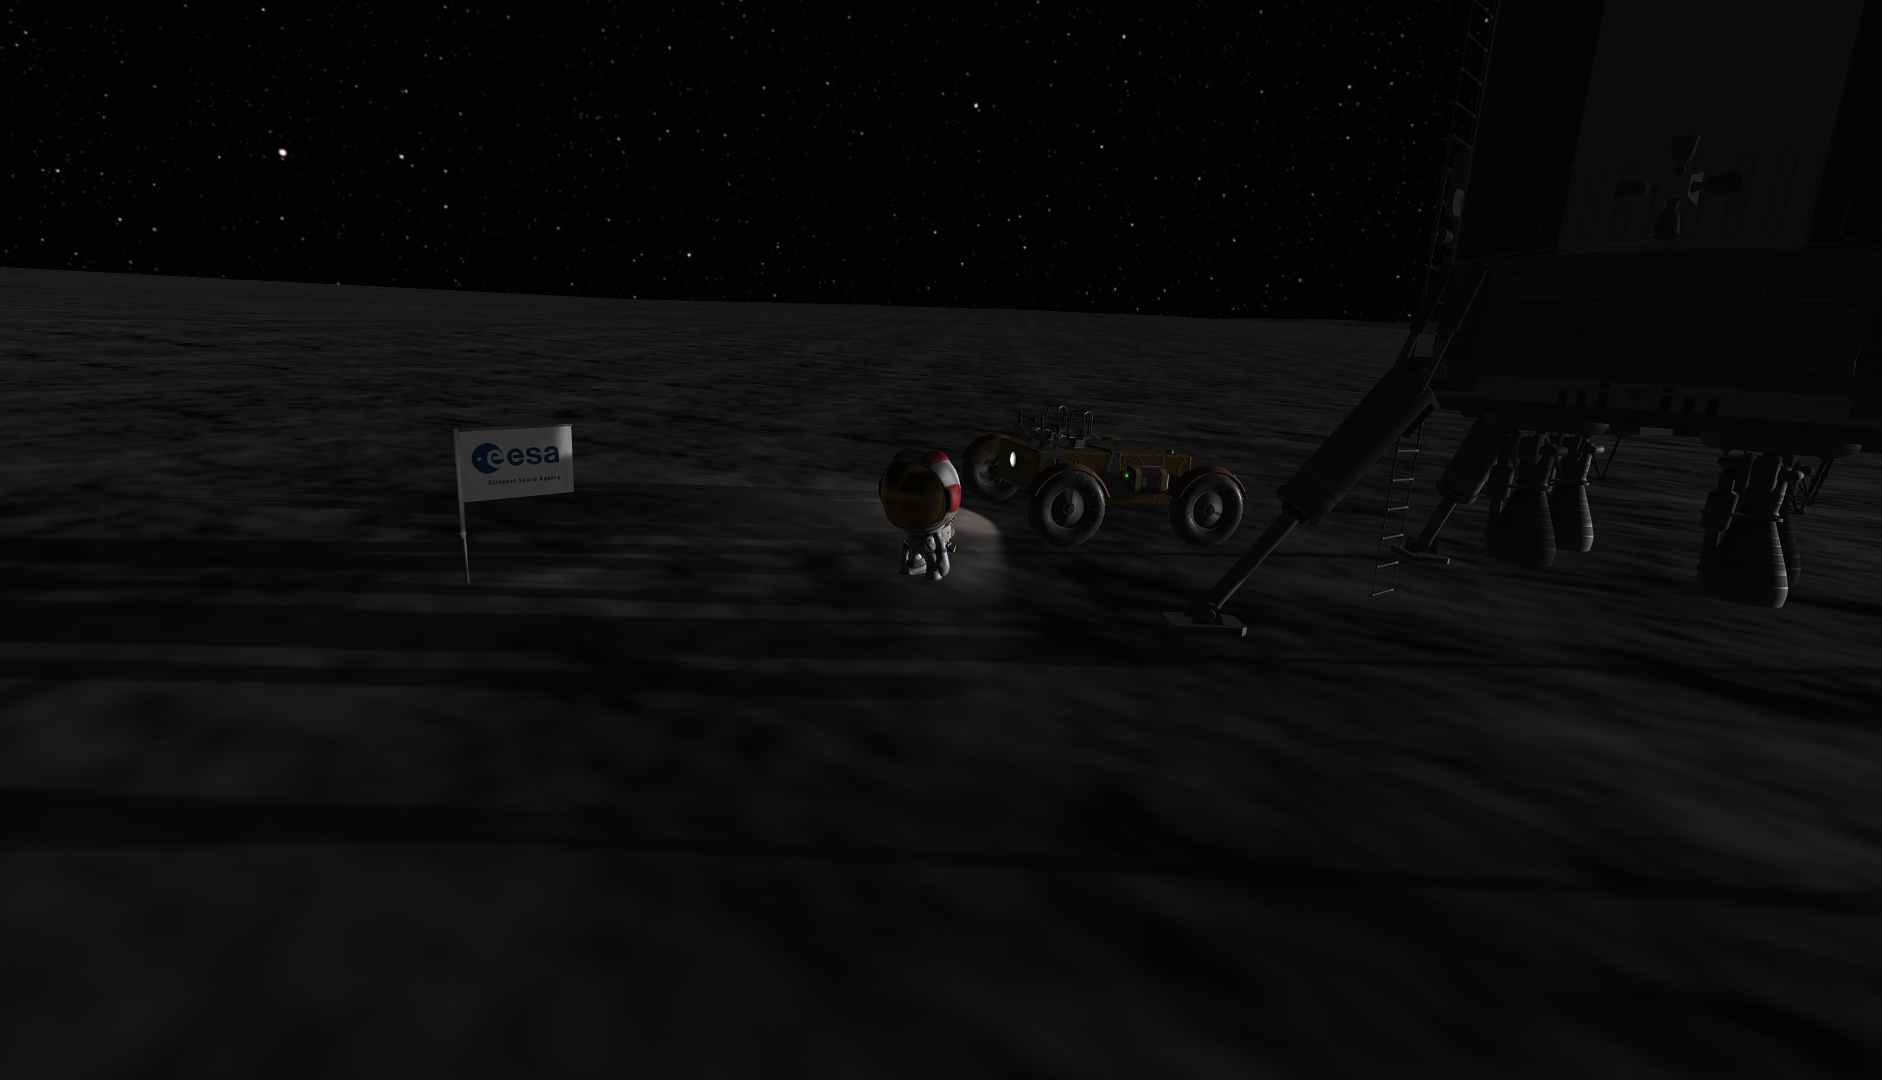
\includegraphics[width=0.8\textwidth]{../assets/Moho/Budapest-I-arrival.png}
    \caption{From left to right: the ESA flag, Dezer Kerman, the
      Columbus rover and the DEL lander in Dezer Crater, shortly after
      landing.}
\end{figure}
\begin{figure}[h]
    \centering
    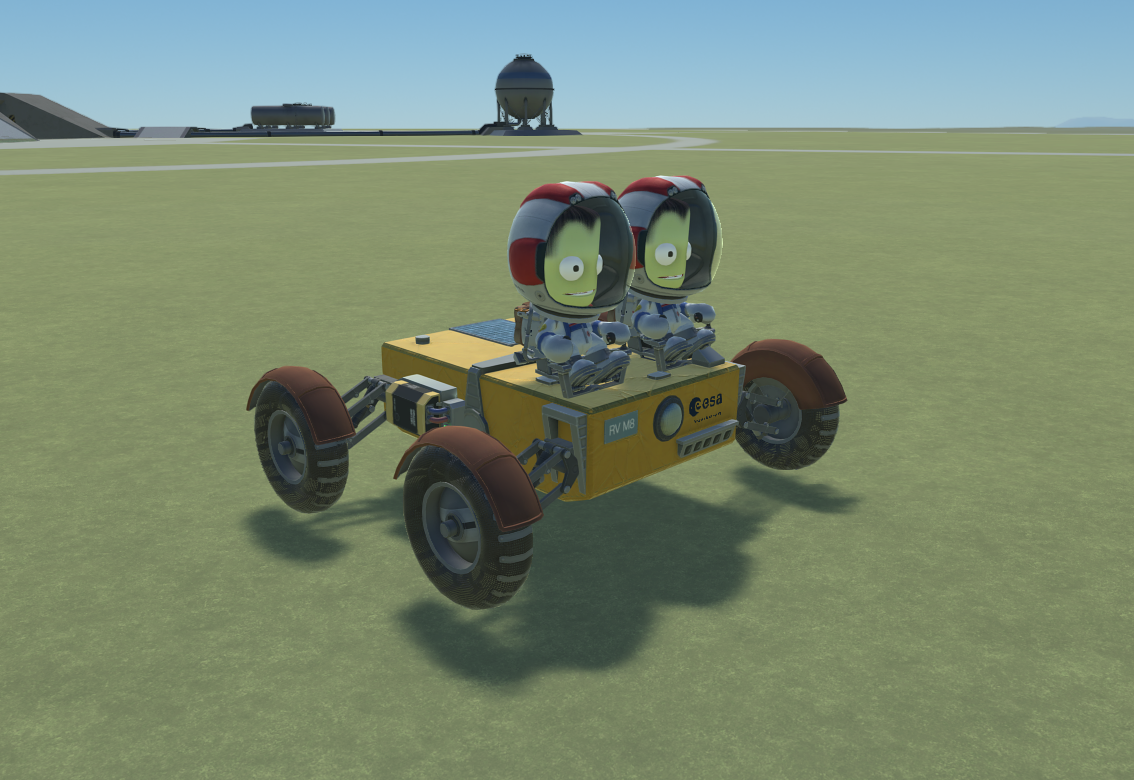
\includegraphics[width=0.8\textwidth]{../assets/Moho/Columbus-test.png}
    \caption{Testing the Columbus rover on Kerbin without the antenna
      and the radioisotope electric generator.}
\end{figure}

\end{document}
